\chapter{Prototype Board Design}
\label{ch:board_design}

\section{Overview}
\label{sec:board_design_overview}

Chapter \ref{ch:topologies} introduced the FWR and NVC rectifier topologies used in this thesis, and Chapter \ref{ch:simulations} evaluated their Simulink models. This chapter describes the prototype board built to test these topologies on the real MP-VREH harvester, from the component choices behind it to its schematic and physical layout.

\section{Components Used}
\label{sec:components_used}

Both the FWR and NVC stages of Chapter \ref{ch:topologies} are built on prototype boards using the components listed in Table \ref{tab:board_components}. The same Schottky diode part is used for every diode across both bridges, whether as the FWR's own rectifying diodes or as the parallel diodes of the NVC's cross-coupled bridge, and this bridge itself is built from two N-MOSFETs and two P-MOSFETs. As discussed in Section \ref{sec:nvc}, the critical voltage $V_\text{off}\approx1.2\ \text{V}$ below which the NVC bridge falls back to diode conduction is set by the largest threshold voltage among its four MOSFETs; Table \ref{tab:board_components} shows that this is the N-MOSFET's $V_\text{GS(th)}=1.2\ \text{V}$, larger in magnitude than the P-MOSFET's $V_\text{GS(th)}=-1.0\ \text{V}$.

\begin{table}[htbp]
    \centering
    \begin{tabular}{lll}
        \toprule
        Component & Specification & Characteristics \\
        \midrule
        $D_1$--$D_{10}$ & Schottky diode (CTS05S40-L3F) & $V_F=0.31\ \text{V}$ @ $I_F=0.1\ \text{A}$ \\
        $N_1$, $N_2$ & N-MOSFET (BSS138PW-115) & $R_\text{DSon}=1\ \Omega$, $V_\text{GS(th)}=1.2\ \text{V}$, $V_\text{SD}=0.75\ \text{V}$ \\
        $P_1$, $P_2$ & P-MOSFET (PMN27XPE-115) & $R_\text{DSon}=27\ \text{m}\Omega$, $V_\text{GS(th)}=-1.0\ \text{V}$, $V_\text{SD}=-0.7\ \text{V}$ \\
        \bottomrule
    \end{tabular}
    \caption{Key components used on the FWR and NVC prototype boards.}
    \label{tab:board_components}
\end{table}

\section{Schematic}
\label{sec:board_schematic}

Figures \ref{fig:board_sch_p1}--\ref{fig:board_sch_p6} show the complete schematic of the prototype board, page by page. The board integrates both FWR three-phase groups (FBR1, FBR2) and all three NVC bridges (NVC1--NVC3), together with jumpers that reconfigure each coil between the FWR and NVC paths, the FWR groups between star and delta connection, and the compensation capacitor $C_m$ of each coil, so that every configuration simulated in Chapter \ref{ch:simulations} can be tested on the same board.

\begin{figure}[h!]
    \centering
    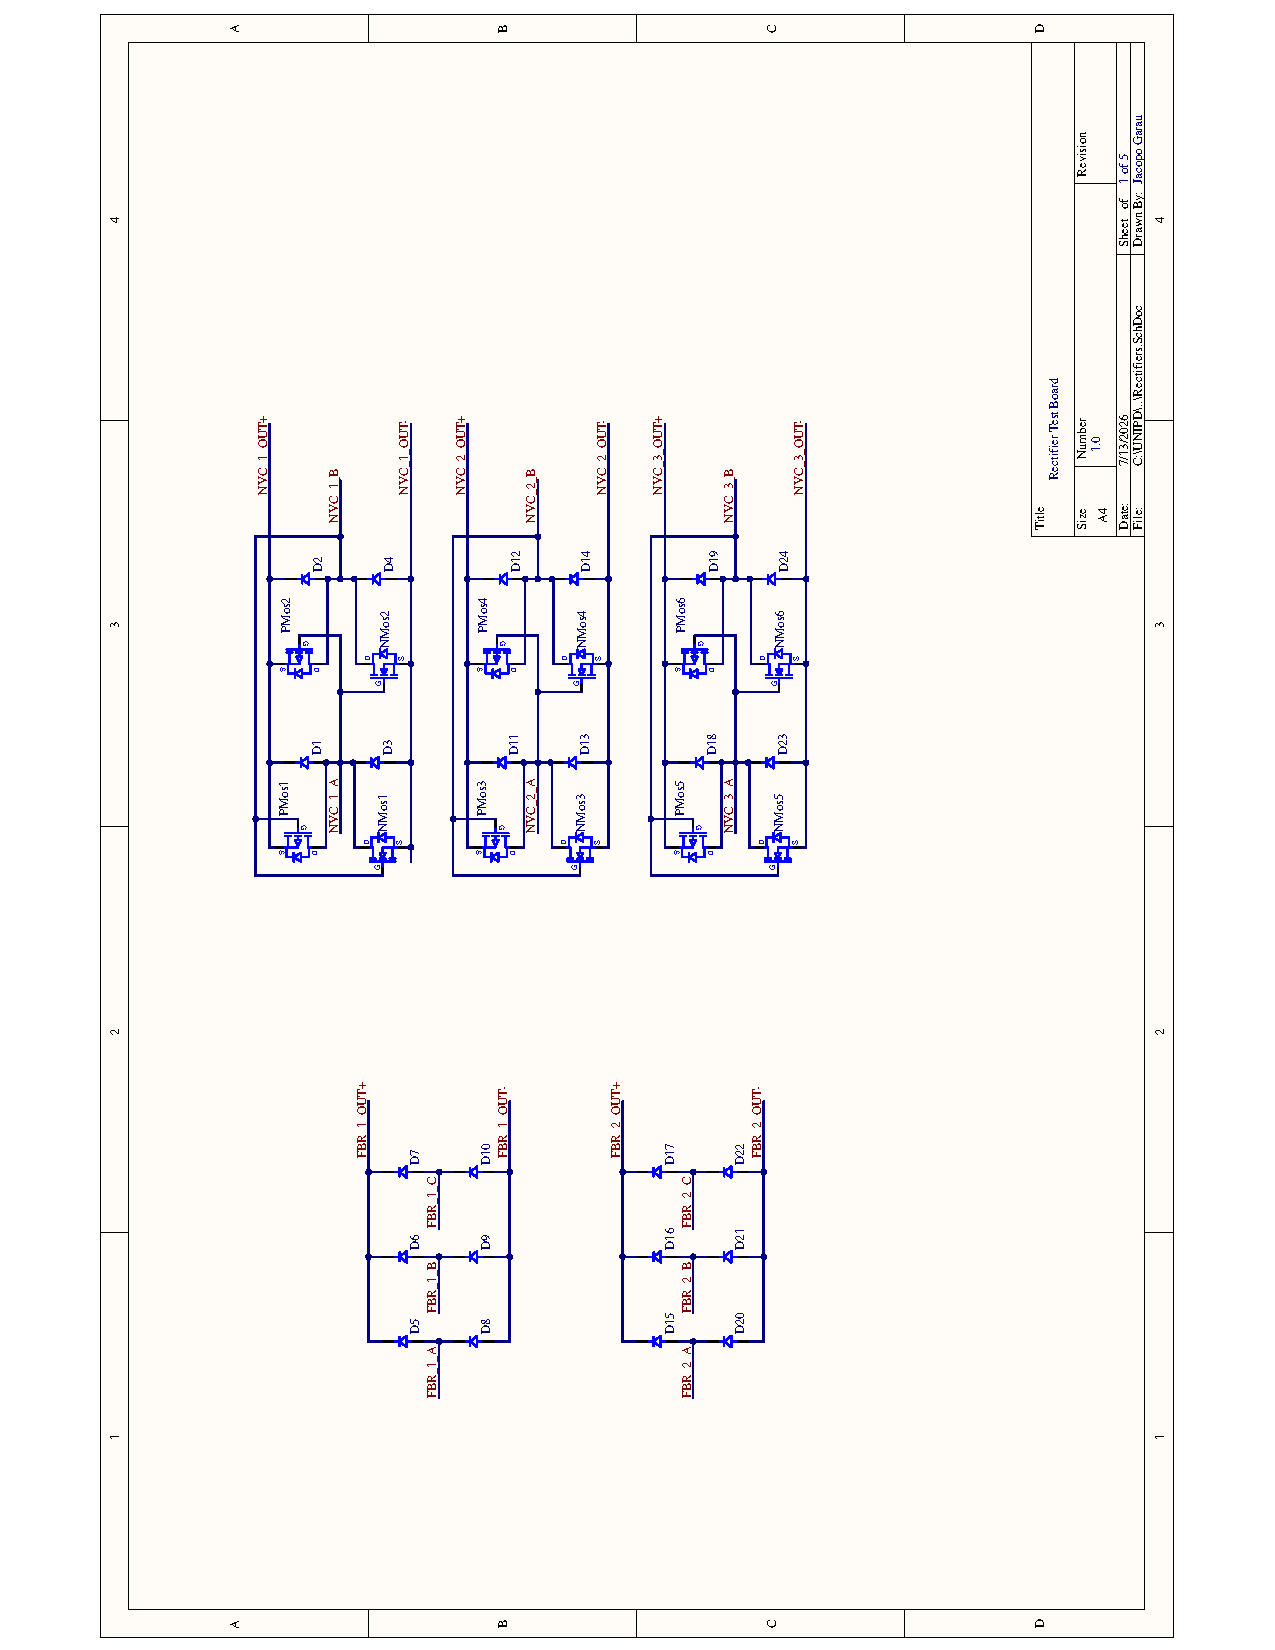
\includegraphics[page=1, width=0.95\textwidth]{Circuits/Rectifiers_Board_rotated.pdf}
    \caption{Rectifier bridges: the two FWR three-phase groups (FBR1, FBR2) and the three anti-series NVC bridges (NVC1--NVC3).}
    \label{fig:board_sch_p1}
\end{figure}

\begin{figure}[h!]
    \centering
    \includegraphics[page=2, width=0.95\textwidth]{Circuits/Rectifiers_Board_rotated.pdf}
    \caption{Common connectors: input connectors for the six coils, current-sensing measurement points, and the jumpers selecting whether each coil feeds the FWR or the NVC bridges.}
    \label{fig:board_sch_p2}
\end{figure}

\begin{figure}[h!]
    \centering
    \includegraphics[page=3, width=0.95\textwidth]{Circuits/Rectifiers_Board_rotated.pdf}
    \caption{FWR connections: jumpers selecting the star or delta connection of each three-phase group, the output filter capacitors, and the bridge and output voltage measurement points.}
    \label{fig:board_sch_p3}
\end{figure}

\begin{figure}[h!]
    \centering
    \includegraphics[page=4, width=0.95\textwidth]{Circuits/Rectifiers_Board_rotated.pdf}
    \caption{NVC connections: anti-series pairing of the six coils, the output filter capacitors, and the voltage measurement points for the three NVC bridges.}
    \label{fig:board_sch_p4}
\end{figure}

\begin{figure}[h!]
    \centering
    \includegraphics[page=5, width=0.95\textwidth]{Circuits/Rectifiers_Board_rotated.pdf}
    \caption{Matching capacitors: the jumper-selectable parallel capacitor bank used to set the compensation capacitor $C_m$ of each coil.}
    \label{fig:board_sch_p5}
\end{figure}

\begin{figure}[h!]
    \centering
    \begin{subfigure}{0.85\textwidth}
        \includegraphics[page=6, width=\textwidth]{Circuits/Rectifiers_Board_rotated.pdf}
        \caption{Bottom copper layer.}
    \end{subfigure}

    \begin{subfigure}{0.85\textwidth}
        \includegraphics[page=7, width=\textwidth]{Circuits/Rectifiers_Board_rotated.pdf}
        \caption{Top copper layer.}
    \end{subfigure}
    \caption{PCB layout: bottom (a) and top (b) copper layers.}
    \label{fig:board_sch_p6}
\end{figure}
